\chapter{Modellazione e Risultati \label{cap5}}
In questa sezione sono presentati i principali aspetti per
ottenere un modello del reattore ALFRED il più possibile vicino al modello
preliminare proposto dal progetto LEADER. Sono descritte le principali
approssimazione delle simulazioni.
Inoltre sono mostrati i risultati ottenuti in funzione delle variazioni di 
temperatura
del combustibile, dei tempi di bruciamento e dell'inserimento dei sistemi di 
sicurezza.
I risultati vertono principalmente sulla distribuzione di flusso neutronico, di 
potenza termica
e di temperatura e sono ottenuti attraverso le capacità offerte dall'accoppiamento neutronico-termoidraulico della piattaforma numerica, descritta nel Capitolo \ref{cap4}.

\section{Modellazione del reattore ALFRED \label{modelalfred}}

Al fine di modellare correttamente il reattore nucleare, è necessario
curare con precisione ogni suo elemento.
Viene descritta soprattutto la costruzione delle sezioni d'urto macroscopiche del singolo assembly di combustibile, la quale risulta di 
fondamentale importanza
per la validità del calcolo neutronico dell'intero reattore.
La geometria e l'assegnazione dei vari elementi che compongono l'intero 
reattore 
risulta anch'essa di fondamentale importanza per la corretta simulazione
del reattore in questione.

\subsection{Elemento di combustibile}

%%%%%%%%%%%%%%%%%%%%%%%%%%%%%%%%%%%%%%%%%%%%%%%%%%%%%%%%%%%%%%%%%%%%5
\begin{figure}[!htb]
\centering
\subfigure[Assembly di combustibile. \label{fassembly}]
{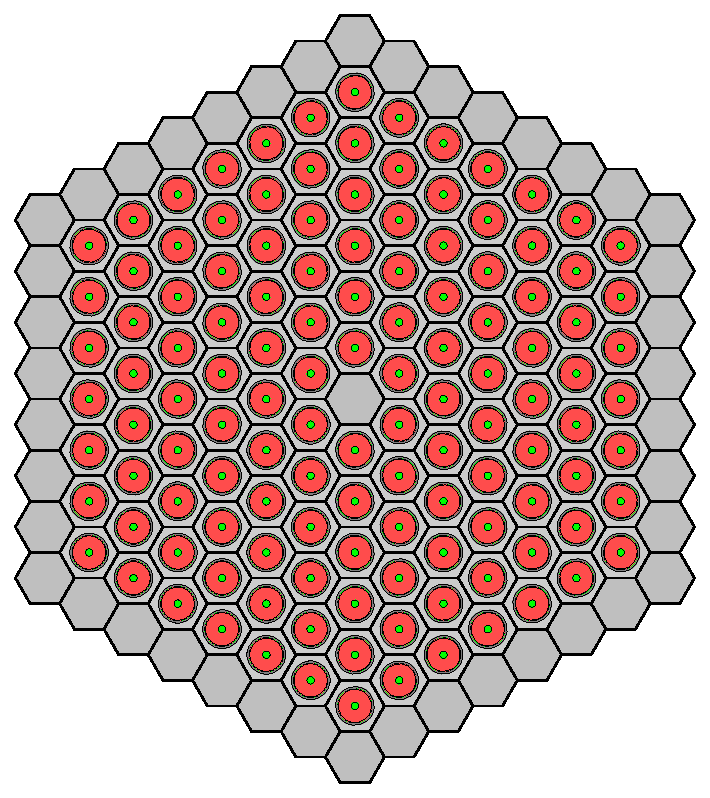
\includegraphics[width=0.48\textwidth]{./figure/itex/fassembly}}
\centering
\subfigure[Elemento di combustibile. \label{unitcells}]
{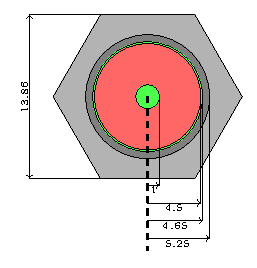
\includegraphics[width=0.48\textwidth]{./figure/itex/unitcells_wq}}
\caption{Modello dell'assembly di combustibile al fine di creare il database 
per il combustibile. }
\end{figure}
%%%%%%%%%%%%%%%%%%%%%%%%%%%%%%%%%%%%%%%%%%%%%%%%%%%%
\begin{table}[!htb]
\centering
 \begin{tabular}{lcc}
\toprule
Parametro & Unità & Valore \\
\midrule
Numero totale di esagoni & - & 169 \\
Numero di barre di combustibile & - & 126 \\
Numero di elementi di acciaio & - & 43 \\
Lato di un esagono & mm & 8.00208 \\
Apotema di un esagono & mm & 6.93 \\
Distanza tra barre di combustibile & mm & 13.86 \\
Raggio totale della barra di combustibile & mm & 5.25 \\
\bottomrule
\end{tabular}
\caption{Parametri di modellazione in riferimento all'assembly di combustibile 
in Figura \ref{fassembly}. \label{tabcrosection}}
\end{table}
%%%%%%%%%%%%%%%%%%%%%%%%%%%%%%%%%%%%%%%%%%%%%%%%%%%%%%%%%%
%%%%%%%%%%%%%%%%%%%%%%%%%%%%%%%%%%%%%%%%%%%%%%%%%%%%%%5
\begin{table}[!htb]
\small
\centering
 \begin{tabular}{lcccccccc}
 \toprule
 Parametro & Unità & Valori &  &  &   & & \\
 \midrule
Temperatura del combustibile & [$^\circ$C] & 400.0 & 550.0 & 700.0 & 850.0 & 1000.0 
\\
\midrule
Temperatura del refrigerante & [$^\circ$C] & 380.0 & 440.0 & 600.0 & 750.0 &  \\
\midrule
Valori di bruciamento salvati & [Giorni] & 0.0 & 365.0 & 730.0 & 1095.0 & \\ 
\bottomrule
\end{tabular}
\caption{Dati di ingresso per la creazione del database reattoristico.\label{daticompo}}
\end{table}
%%%%%%%%%%%%%%%%%%%%%%%%%%%%%%%%%%%%%%%%%%%%%%%%%%%%%
La modellazione del reattore ALFRED avviene in primo luogo attraverso la 
creazione del 
database reattoristico, il cui procedimento è descritto nella Sezione 
\ref{datareactor}.
Per la libreria dei dati nucleari, relativi alle sezioni d'urto microscopiche 
dei materiali, 
\`e stata utilizzata la versione 3.1.2SHEM delle \textit{Jeff} a 315 gruppi 
energetici. 
Al fine dei calcoli di reattori, si ottiene il database contenente le sezioni 
d'urto omogeneizzate e condensate a 33 gruppi energetici.

L'assembly di combustibile è costruito secondo una geometria esagonale a due 
dimensioni
composte da celle esagonali che contengono la singola barra di combustibile o 
l'elemento strutturale, come in Figura \ref{fassembly}.
La singola cella esagonale rappresentata in Figura \ref{unitcells} è costituita 
dalla 
sezione della barra di combustibile immersa nel piombo refrigerante. La barra 
di combustibile è modellata con una geometria circolare (pin) ed è composta da 
una pastiglia cava
di combustibile MOX e dalla guaina di rivestimento in una lega di acciaio 
denominata 15-15 Ti AIM1 \cite{angiolini2017specifica}.
All'interno della cavità della pastiglia e nel divario tra pastiglia e guaina 
di 
rivestimento è contenuto il gas inerte di fissione, in questo caso elio.
I parametri dimensionali per la modellazione sono stati ricavati dal modello di 
riferimento dell'assembly 
di combustibile del reattore ALFRED presente nella sezione 
\label{alfredsection}, al fine di mantenere 
la stessa distanza tra due barre di combustibile, e sono mostrati in Tabella 
\ref{tabcrosection}.

Sono stati analizzati i parametri di temperatura del combustibile, del 
refrigerante e i valori di bruciamento 
al fine di creare il database complessivo richiesto 
per l'interpolazione dal codice di reattore, tabulati in Tabella 
\ref{daticompo}.
Inoltre il valore di potenza termica lineare, di ogni assembly di 
combustibile, per il calcolo del bruciamento del combustibile ad ogni step 
temporale è stato impostato a $40$W/g. Questo permette l'andamento dei valori 
di potenza termica rilasciata  bruciamento del combustibile.


\subsection{Reattore complessivo}

%%%%%%%%%%%%%%%%%%%%%%%%%%%%%%%%%%%%%%%%%%%%%%%%%%%%%%%%%%%%%%%%%
\begin{figure}[!htb]
 \centering
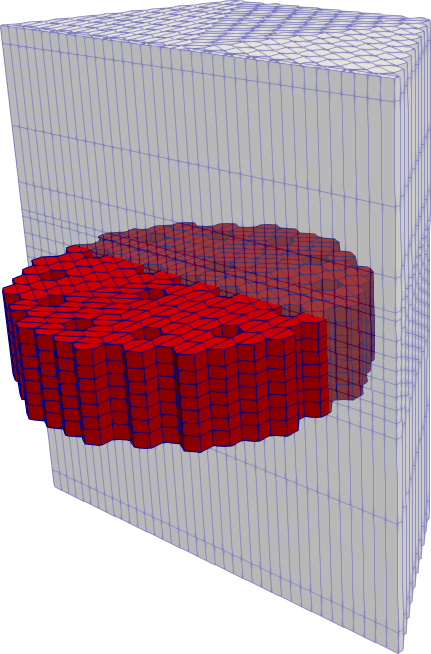
\includegraphics[scale=0.35]{./figure/result_tred/new/tred-reactor.png}
\caption{Rappresentazione tridimensionale del reattore ALFRED, dove è evidenziato in rosso il 
nocciolo.\label{modellotredalfred}}
\end{figure} 
%%%%%%%%%%%%%%%%%%%%%%%%%%%%%%%%%%%%%%%%%%%%%%%%%%%%%%%%%%
%%%%%%%%%%%%%%%%%%%%%%%%%%%%%%%%%%%%%%%%%%%%%%%%%%%%%%%%%%%%%%%%%%%%%%%%%%%%%%%%
%55
\begin{table}[!htb]
\small
\centering
 \begin{tabular}{lcc}
\toprule
Parametro & Unità & Valore \\
\midrule
Lato elemento esagonale & cm & 9.87269 \\
Apotema elemento esagonale & cm & 8.5500 \\
Numero totale di elementi esagonali & - & 271 \\ 
Numero di assembly di combustibile totali & - & 134 \\
Numero di assembly di combustibile interne & - & 56 \\
Numero di assembly di combustibile totali & - & 78 \\
Numero di barre di controllo & - & 12 \\
Numero di barre di sicurezza & - & 4 \\
Numero di elementi strutturali & - & 121 \\
Arricchimento MOX interno & $\%$ & 20.5 \\
Arricchimento MOX esterno & $\%$ & 26.2 \\
\bottomrule
\end{tabular}
\caption{Parametri del modello di nocciolo intesi per piano.}
\label{nocciolo}
\end{table}
%%%%%%%%%%%%%%%%%%%%%%%%%%%%%%%%%%%%%%%%%%%%%%%%%%%%%%%%%%%%%%%%%%%%%%%%%%%%%
\Figure[scale=0.5]{./figure/itex/hexagon}{Configurazione radiale del modello 
di 
ALFRED utilizzato nel calcolo neutronico di reattore.}{hexagon}
\Figure[scale=0.5]{./figure/itex/rectangle_wq}{Configurazione assiale del 
modello 
di ALFRED utilizzato nel calcolo neutronico di reattore.}{rectangle}
%%%%%%%%%%%%%%%%%%%%%%%%%%%%%%%%
\begin{figure}[!htb]
\centering
\subfigure[Conducibilità termica mediata \label{tempeq}]
{
\includegraphics[height=0.3\textheight]{./figure/itex/tempeq}}
\hspace{5mm}
\subfigure[Canale chiuso \label{canale}]
{
\includegraphics[height=0.3\textheight]{./figure/itex/canale}}
\caption{Principali approssimazione considerate per la risoluzione termoidraulica di ciascun elemento del reattore.}
\end{figure}
%%%%%%%%%%%%%%%%%%%%%%%%%%%%%%%%
\begin{table}[!htb]
\centering
 \begin{tabular}{lccc}
\toprule
Parametro & Simbolo & Unità & Valore \\
\midrule
Densità & $\rho$ & kg/m$^3$ & 11340 \\
Conduttività termica & $\lambda$ & W/(m$\cdot$K) & 35 \\
Calore specifico & $c_p$ & J/(kg$\cdot$K) & 129 \\
Viscosità dinamica & $\mu$ & Pa$\cdot$s & 0.001844 \\
\bottomrule
\end{tabular}
\caption{Principali parametri termodinamici che caratterizzano il piombo 
liquido.}
\label{leadparam}
\end{table}
%%%%%%%%%%%%%%%%%%%%%%%%%%%%%%%%%%%%%%%%%%%%%%%%%%%%%%%
In Figura \ref{modellotredalfred} è mostrato il modello tridimensionale di 
ALFRED con la corrispondente mesh, dove il nocciolo del reattore è 
evidenziato in rosso.
La geometria tridimensionale è modellata come un prisma esagonale, composto a 
sua volta da altri elementi esagonali.
La struttura radiale del nocciolo è composta come in Figura \ref{hexagon}:
l'esagono è composto in totale da 271 esagoni suddivisi nei
diversi componenti del reattore.
Sono presenti 134 elementi di combustibile agli ossidi misti di cui 56 interni 
sono arricchiti 
al 20.5$\%$ in plutonio $^{239}Pu$ (in giallo) mentre i restanti 78 esterni sono 
arricchiti
al 26.2$\%$ (in rosso).
Inoltre sono 
presenti 4 barre di sicurezze (in viola) e 12 barre di controllo (in verde), 
le quali potranno essere 
inserite e valutarne l'efficienza dei sistemi di controllo della reattività.
Allo stesso modo sono definiti 16 piani che compongono il reattore secondo lo 
schematico di Figura \ref{rectangle} che rappresenta la modellazione assiale 
del 
reattore.
La zona attiva del reattore, 
ovvero la regione in cui è contenuto il combustibile fissile, ha dimensioni 
pari a 60cm; questa zona contiene 7 piani 
per approfondire il calcolo in questa regione, ottenendo così 938 elementi di 
combustibile.
Nella zona attiva, i diversi arricchimenti di combustibile hanno lo scopo di rendere più 
uniforme il flusso neutronico (flat flux). I parametri più importanti relativi 
alla sezione radiale della zona in cui è presente il combustibile 
sono riportati in Tabella \ref{nocciolo}.
L'elemento centrale, che attraversa tutto il reattore, costituisce il 
cosiddetto 
\textit{in-pile} (in blu) mentre sono presenti
sopra e sotto al reattore le zone in cui si accumula il piombo refrigerante, 
\textit{plenum} (in grigio), e le griglie per l'alloggiamento delle assembly 
di combustibile.
Infine sono stati modellati i riflettori ed elementi che svolgono la funzione 
di 
protezione neutronica e posizionati nelle zone più esterne 
del reattore.
La potenza termica totale rilasciata dal reattore è pari a 300MW$_{th}$ ed è 
ottenuta
dal codice di neutronica attraverso la risoluzione delle equazioni $SP_N$ del 
flusso neutronico sopra l'intero
reattore. La potenza termica è trasferita negli elementi computazionali del 
codice di termoidraulica al
fine di ottenere la distribuzione di temperatura.

Dal punto di vista termoidraulico, la simulazione risulta 
semplificata da diverse approssimazioni.
Il modello radiale è stato considerato in 
modo 
che il termine di conducibilità
termico dei singoli sia mediato sulla conducibilità termica del piombo, come 
descritto dalla Figura \ref{tempeq}.
Inoltre le diverse assembly sono stati considerati come canali chiusi attraversati 
dal 
fluido refrigerante, con una velocità costante uguale
a 1.28m/s. Una descrizione del modello è mostrata in Figura \ref{canale}.
In Tabella \ref{leadparam} sono elencati i più importanti parametri 
termodinamici che caratterizzano il piombo come fluido refrigerante e che
sono stati utilizzati durante la simulazione del reattore.
La risoluzione del campo di temperatura è trasferita al modulo neutronico al 
fine di correggere le sezioni d'urto mediate 
a seguito delle variazioni di temperatura del combustibile.
Viene così attuato un ciclo iterativo che garantisce l'evoluzione del reattore 
per tempi di bruciamento assegnati. L'accoppiamento tra neutronica e termoidraulica
è garantita dalla piattaforma numerica attraverso lo scambio delle strutture dati.


\section{Valutazione dei risultati}
I risultati ottenuti sono presentati in questa sezione, attraverso grafici che confrontano
diversi parametri e attraverso la visualizzazione tridimensionale delle distribuzioni di flusso neutronico, di potenza termica 
e di temperatura sull'intero reattore.

\subsection{Valutazione neutronica del modello di ALFRED}

%%%%%%%%%%%%%%%%%%%%%%%%%%%%%%%%%%%%%%%%%%%%%%%%%
\begin{figure}
\centering
\subfigure[$k_{eff}$ \label{keff_in_out_side0}]
{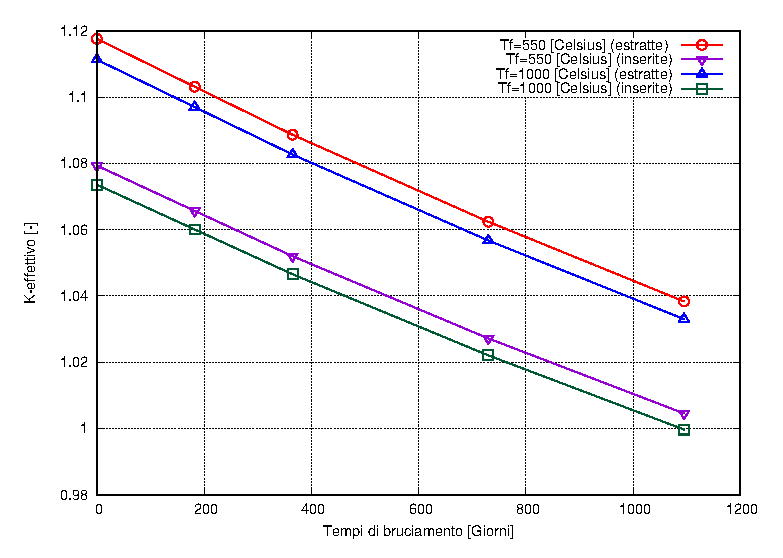
\includegraphics[width=0.48\textwidth]{./graph/keff_in_out_side0}}
% \hspace{5mm}
\subfigure[$\Delta \rho$ \label{reatt_burnup}]
{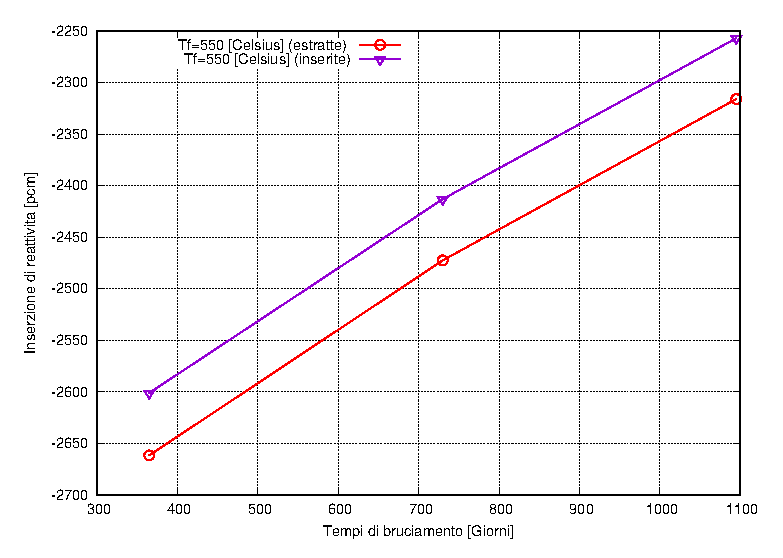
\includegraphics[width=0.48\textwidth]{./graph/reatt_burnup}}
\caption{Costante moltiplicativa effettiva (a) e variazione di reattività (b) in funzione dei tempi di 
bruciamento.}
\end{figure}
%%%%%%%%%%%%%%%%%%%%%%%%%%%%%%%%%%%%%%%%%%%%%%%%%%%%%%%%%%%%%%
\begin{table}[!htb]
\centering
 \begin{tabular}{l|cc|cc}
\toprule
Tempo [Giorni] & $k_{eff}$ Donjon [-] & & $k_{eff}$ MCNPX [-] & \\
 & Barre Inserite & Estratte & Barre Inserite & Estratte \\
\midrule
0   & 1.07935& 1.1177  & 1.0525 & 1.0804 \\
365 & 1.0520 & 1.0887  & 1.0229 & 1.0510   \\
730 & 1.0272 & 1.0624  & 0.9964 & 1.0247   \\
1095 & 1.0001 & 1.0384 & 0.9703 & 0.9988  \\
\bottomrule
\end{tabular}
\caption{Confronto tra valori di $k_{eff}$ nel codice deterministico Donjon e 
quello probabilistico MCNPX.}
\label{keff_su_burn}
\end{table}
%%%%%%%%%%%%%%%%%%%%%%%%%%%%%%%%%%%%%%%%%%%%%%%%%%%%%%%%%%%%%%
\begin{figure}[!htb]
\centering
\subfigure[$k_{eff}$ \label{keff_temp}]
{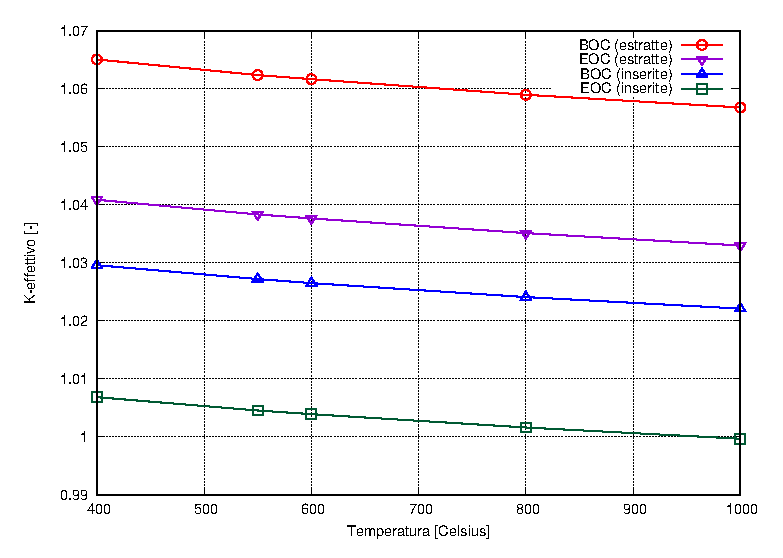
\includegraphics[width=0.48\textwidth]{./graph/keff_temp}}
% \hspace{5mm}
\subfigure[$\Delta \rho$\label{reatt_doppler}]
{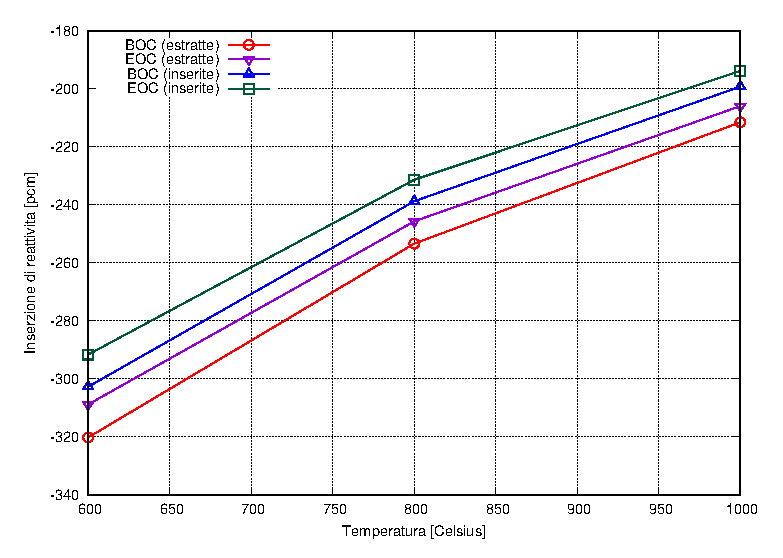
\includegraphics[width=0.48\textwidth]{./graph/reatt_doppler}}
\caption{Costante moltiplicativa effettiva (a) e variazione di reattività (b) in funzione delle 
variazioni di temperatura del combustibile.}
\end{figure}
%%%%%%%%%%%%%%%%%%%%%%%%%%%%%%%%%%%%%%%%%%%%%%%%%%%%%%%%%%%%

La valutazione neutronica del modello di ALFRED, così costruito, avviene sui 
parametri relativi alla costante moltiplicativa effettiva $k_{eff}$ e al 
coefficiente  di 
reattività durante la variazione di altri parametri come la temperatura del 
combustibile $T_f$, dovuto alla modifica delle sezioni d'urto per effetto 
Doppler, e i tempi di bruciamento, dovuti all'evoluzione isotopica all'interno 
del combustibile o durante l'inserimento delle barre di controllo.
La variazione del coefficiente di reattività è espressa in unità pcm (per centomila) e 
determinata dalla formula
\begin{equation}
 \Delta \rho = \frac{\Delta k_{eff}}{k_{eff}} \,.
\end{equation}
Inoltre sono considerati i tempi di inizio ciclo (BOC) a 2 anni e di fine ciclo 
(EOC) a 3 anni. In teoria dopo questo tempo il combustibile fissile, che man 
mano si esaurisce, dovrebbe essere rimpiazzato da altro fissile attraverso la 
trasmutazione degli isotopi fertili.

Nel grafico di Figura \ref{keff_in_out_side0} si nota come l'andamento del 
$k_{eff}$ sia decrescente in quanto durante l'evoluzione del reattore nel tempo 
avviene un processo di bruciamento del combustibile fissile che porta ad una 
diminuzione delle reazioni di fissioni.
Pertanto questo andamento, tabulato in Tabella \ref{keff_su_burn}, è 
confrontato 
con un altro studio effettuato con il codice MonteCarlo, MCNPX, presente nello 
studio \cite{rocchi2013d07} da cui si nota un piccolo scostamento dovuto sia a 
differenze intrinseche tra i metodi deterministi e probabilistici, sia a 
piccole 
differenze tra i modelli del reattore usati.
Tuttavia la variazione di reattività durante l'evoluzione del combustibile nel 
tempo è in linea con il processo di decadimento del combustibile e rasserena di 
aver costruito correttamente le sezioni d'urto presenti nel database 
reattoristico, presentata nel grafico di Figura \ref{reatt_burnup}.

Nei grafici di Figura \ref{keff_temp} e \ref{reatt_doppler}, sono mostrati gli 
andamenti in funzione della temperatura del combustibile. Si nota che ad un 
aumento di temperatura, il $k_{eff}$ diminuisce per effetto Doppler, il quale è 
molto importante nella valutazione del coefficiente di temperatura $\alpha_T$ e 
quindi della regolazione del reattore stesso.
Infatti questo termine è negativo e permette una inserzione negativa di 
reattività diminuendo così le reazioni di fissioni in maniera praticamente 
istantanea. Questo effetto con l'aumentare della temperatura è meno accentuato.
Sono stati valutati i risultati ottenuti in funzione dell'inserimento delle barre 
di controllo. 
Le inserzioni di reattività dovute all'inserimento delle barre di controllo 
risultano in media pari a -3453.574pcm. Tuttavia non è stato analizzato il 
comportamento dei sistemi di sicurezza a seguito di variazioni di temperatura, 
in quanto sarebbe necessaria un analisi più approfondita sui sistemi di 
sicurezza.

\subsection{Valutazione a fine ciclo (EOC)}
%%%%%%%%%%%%%%%%%%%%%%%%%%%%%%%%%%%%%%%%%%%%%%%%%%%%%%%
\begin{table}[!htb]
\centering
 \begin{tabular}{lccc}
\toprule
Parametro & Unità & Barre inserite & Barre estratte \\
\midrule
$k_{eff}$ & - & 1.0068 & 1.0409 \\
Flusso medio sul reattore & - & 6.5099$\cdot$10$^{12}$ & 6.6889$\cdot$10$^{12}$ 
\\
Potenza totale & MW & 297.627 & 297.289 \\
Potenza media assemblies & kW & 314.2 & 313.4 \\
Potenza media channels & kW & 2221.1 & 2218.6 \\
Densità media di potenza & MW/cm$^3$ & 12.4899626 & 12.4899635 \\
\bottomrule
\end{tabular}
\caption{Valutazione parametri derivati dalla neutronica per il tempo EOC (1095 
giorni). \label{paraminseextr}}
\end{table}
%%%%%%%%%%%%%%%%%%%%%%%%%%%%%%%%%%%%%%%%%%%%%%%%%%%%%%%%%%%%%%%%%%%%
\begin{table}[!htb]
\tiny
\centering
 \begin{tabular}{lccc}
\toprule
Gruppo  & Inizio Intervallo  & Flusso  \\
Energetico & di Energia [eV]  & neutronico medio \\       
\midrule
1 & 1.964 $\cdot$10$^7$  &  5.063305$\cdot$10$^{10}$  \\           
2 & 1.000 $\cdot$10$^7$  &  8.552906$\cdot$10$^{11}$  \\
3 & 6.065 $\cdot$10$^6$  &  4.648414$\cdot$10$^{12}$  \\
4 & 3.679 $\cdot$10$^6$  &  2.666274$\cdot$10$^{13}$  \\
5 & 2.231 $\cdot$10$^6$  &  6.630337$\cdot$10$^{13}$  \\
6 & 1.353 $\cdot$10$^6$  &  8.416610$\cdot$10$^{13}$  \\
7 & 8.209 $\cdot$10$^5$  &  1.851983$\cdot$10$^{14}$  \\
8 & 4.979 $\cdot$10$^5$  &  1.323843$\cdot$10$^{14}$  \\
9 & 3.020 $\cdot$10$^5$  &  1.512711$\cdot$10$^{14}$  \\
10 & 1.831 $\cdot$10$^5$ &  1.405086$\cdot$10$^{14}$  \\
11 & 1.110 $\cdot$10$^5$ &  1.249495$\cdot$10$^{14}$  \\
12 & 6.738 $\cdot$10$^4$ &  1.153978$\cdot$10$^{14}$  \\
13 & 4.087 $\cdot$10$^4$ &  9.083885$\cdot$10$^{13}$  \\
14 & 2.479 $\cdot$10$^4$ &  9.344629$\cdot$10$^{13}$  \\
15 & 1.503 $\cdot$10$^4$ &  7.660485$\cdot$10$^{13}$  \\
16 & 9.119 $\cdot$10$^3$ &  5.569417$\cdot$10$^{13}$  \\
17 & 5.531 $\cdot$10$^3$ &  5.252918$\cdot$10$^{13}$  \\
18 & 3.355 $\cdot$10$^3$ &  4.237772$\cdot$10$^{13}$  \\
19 & 2.034 $\cdot$10$^3$ &  3.361783$\cdot$10$^{13}$  \\
20 & 1.234 $\cdot$10$^3$ &  2.144770$\cdot$10$^{13}$  \\
21 & 7.485 $\cdot$10$^2$ &  1.421856$\cdot$10$^{13}$  \\
22 & 4.540 $\cdot$10$^2$ &  6.478556$\cdot$10$^{12}$  \\
23 & 3.043 $\cdot$10$^2$ &  6.813047$\cdot$10$^{12}$  \\
24 & 1.486 $\cdot$10$^2$ &  1.933539$\cdot$10$^{12}$  \\
25 & 9.166 $\cdot$10$^1$ &  5.600359$\cdot$10$^{11}$  \\
26 & 6.790 $\cdot$10$^1$ &  5.553465$\cdot$10$^{11}$  \\
27 & 4.017 $\cdot$10$^1$ &  3.848728$\cdot$10$^{11}$  \\
28 & 2.260 $\cdot$10$^1$ &  1.812537$\cdot$10$^{11}$  \\
29 & 1.371 $\cdot$10$^1$ &  1.660901$\cdot$10$^{11}$  \\
30 & 8.315 $\cdot$10$^0$ &  1.583113$\cdot$10$^{11}$  \\
31 & 4.000 $\cdot$10$^0$ &  3.292575$\cdot$10$^{11}$  \\
32 & 5.400 $\cdot$10$^{-1}$ & 6.970676$\cdot$10$^{9}$ \\
33 & 1.000 $\cdot$10$^{-1}$ & 2.165139$\cdot$10$^{9}$ \\
Fine Intervallo & 1.100 $\cdot$10$^{-4}$ & \\
\bottomrule
\end{tabular}
\caption{Suddivisioni a 33 gruppi energetici per intervalli di energia e flusso 
neutronico medio all'interno delle zone di combustibile per gruppi di energia. 
\label{groupenergy}}
\end{table}
\Figure[scale=0.8]{./graph/energyy}{Distribuzione del flusso neutronico lungo le 
ordinate all'altezza $z$=175cm per diversi gruppi di energia 
(7, 11, 15, 19, 23, 27).}{energyy}
%%%%%%%%%%%%%%%%%%%%%%%%
\Figure[scale=0.8]{./graph/fluxy}{Distribuzione di flusso lungo l'asse delle 
ordinate all'altezza $z$=175cm confrontando il caso tra barre inserite ed 
estratte.}{graphfluxy}
%%%%%%%%%%%%%%%%%%
\Figure[scale=0.8]{./graph/powery}{Distribuzione di potenza termica lungo l'asse 
delle ordinate all'altezza $z$=175cm confrontando il caso tra barre inserite ed 
estratte.}{graphpowery}
%%%%%%%%%%%%%%%%%%%%%%%%%%%%%%%%%%%%%%%%%%%%%%%%%%%%%%%%%%%%%%%%%%
%%%%%%%%%%%%%%%%%%%%%%%%%%%%%%%%%%%%%%%%%%%%%%%%%%%%%%%%%%%%%%%%%%%%%%%%%%%%%%%%%%%%%%%%%%%%
\begin{figure}[!htb]
\centering
\subfigure[Sezione con barre inserite]
{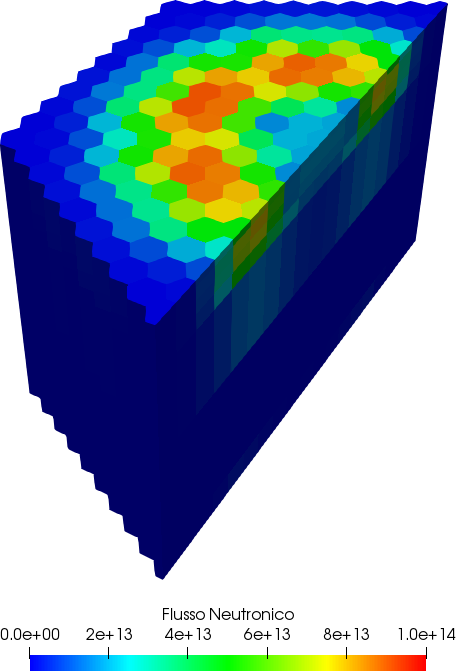
\includegraphics[height=0.3\textheight]{./figure/result_tred/morenew/flux-clip-insert1.png}}
\hspace{1.2cm}
\subfigure[Nocciolo con barre inserite]
{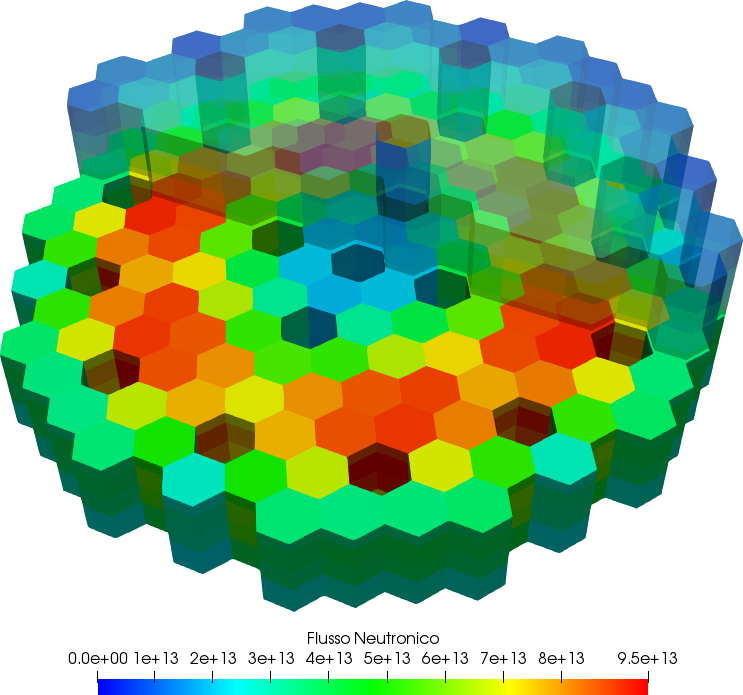
\includegraphics[height=0.3\textheight]{./figure/result_tred/morenew/flux-trashold-insert1.png}}
\\
\subfigure[Sezione con barre estratte]
{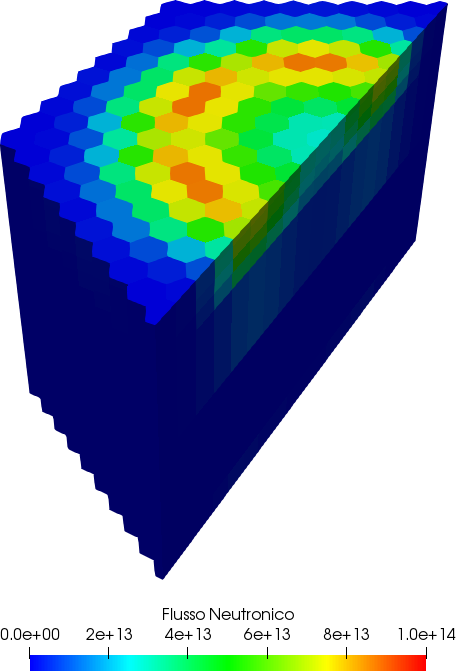
\includegraphics[height=0.3\textheight]{./figure/result_tred/morenew/flux-clip-exstract1.png}}
% % \hspace{5mm}
\hspace{1.2cm}
\subfigure[Nocciolo con barre estratte]
{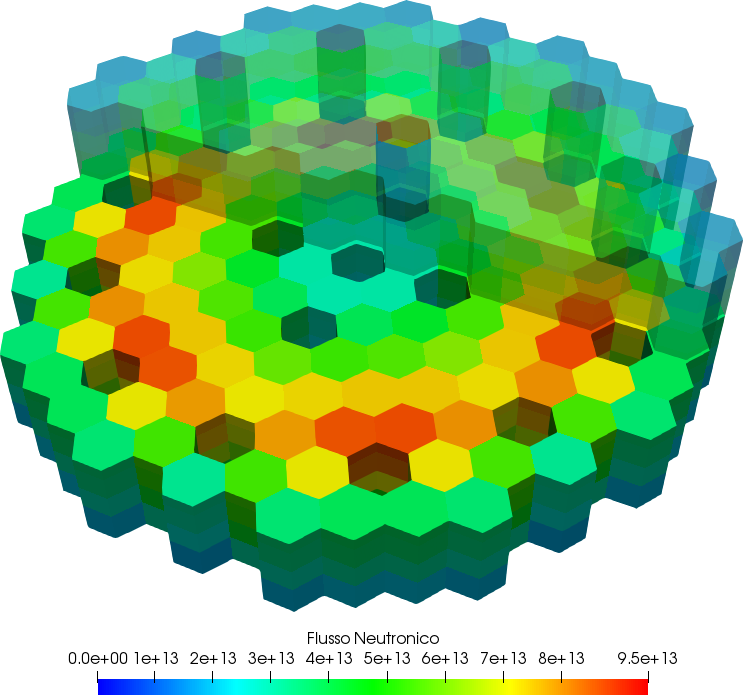
\includegraphics[height=0.3\textheight]{./figure/result_tred/morenew/flux-trashold-exstract1.png}}
\caption{Distribuzione di flusso neutronico sulla sezione radiale del reattore 
(a), (c), e sul nocciolo del reattore (b), (d) in funzione delle barre di 
controllo. \label{nocflux}}
\end{figure}
%%%%%%%%%%%%%%%%%%%%%%%%%%%%%%%%%%%%%%%%
\begin{figure}[!htb]
\centering
\subfigure[Sezione con barre inserite]
{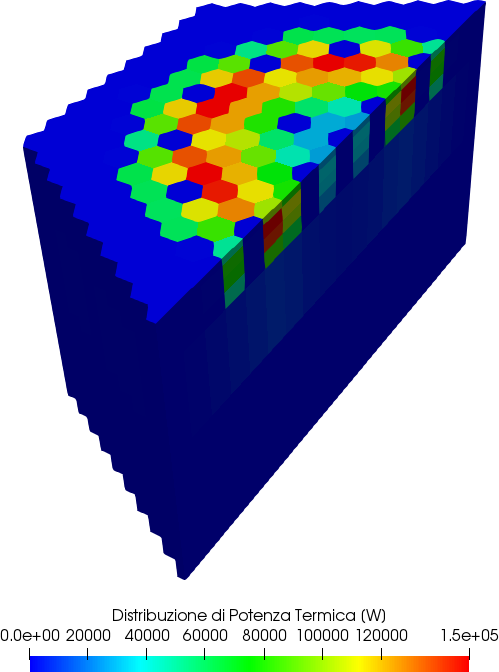
\includegraphics[height=0.28\textheight]{./figure/result_tred/morenew/pw-clip-insert1.png}}
\hspace{1.2cm}
\subfigure[Nocciolo con barre inserite]
{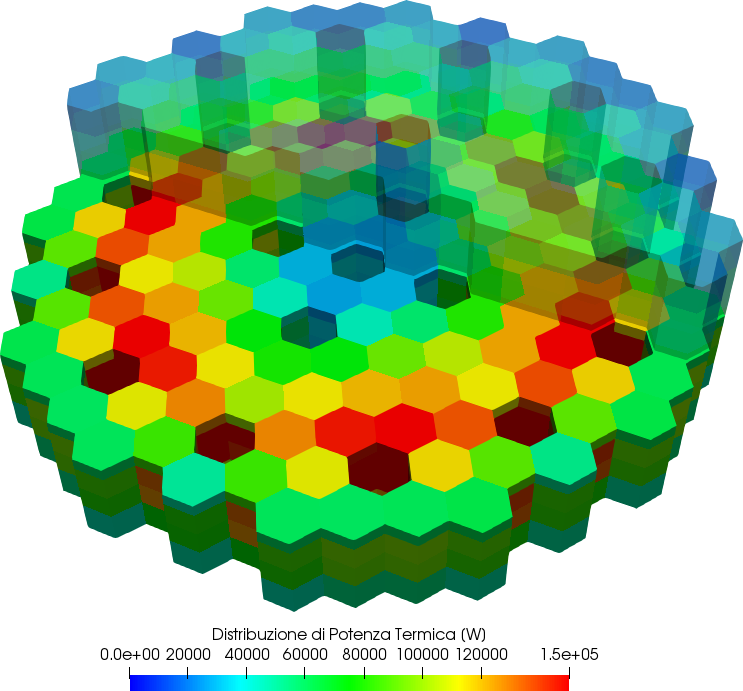
\includegraphics[height=0.28\textheight]{./figure/result_tred/morenew/pw-trashold-insert1.png}}
\subfigure[Sezione con barre estratte]
{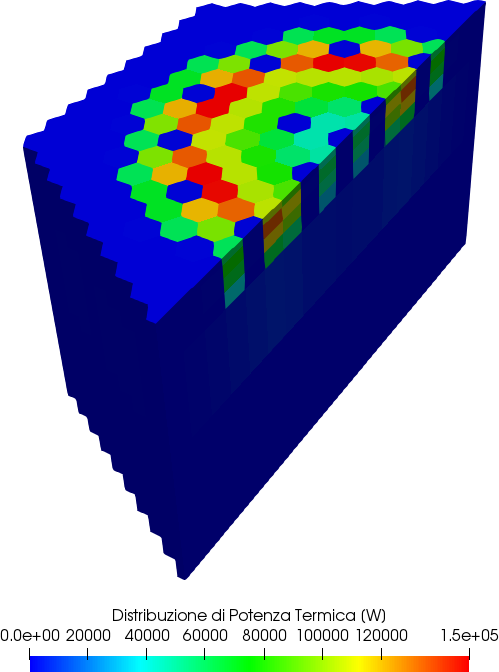
\includegraphics[height=0.28\textheight]{./figure/result_tred/morenew/pw-clip-exstract1.png}}
\hspace{1.2cm}
\subfigure[Nocciolo con barre estratte]
{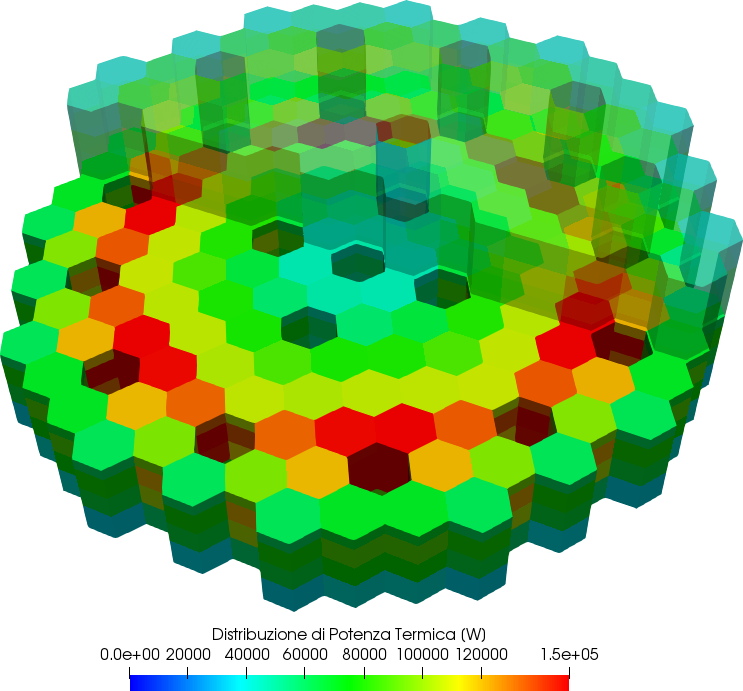
\includegraphics[height=0.28\textheight]{./figure/result_tred/morenew/pw-trashold-exstract1.png}}
\caption{Distribuzione di potenza termica sulla sezione radiale del reattore 
(a), (c), e sul nocciolo del reattore (b), (d) in funzione delle barre di 
controllo. \label{nocpw}}
\end{figure}
%%%%%%%%%%%%%%%%%%%%%%%%%%%%%%%%%%%%%%%
\begin{figure}[!htb]
\centering
\subfigure[Step temporale 1]
{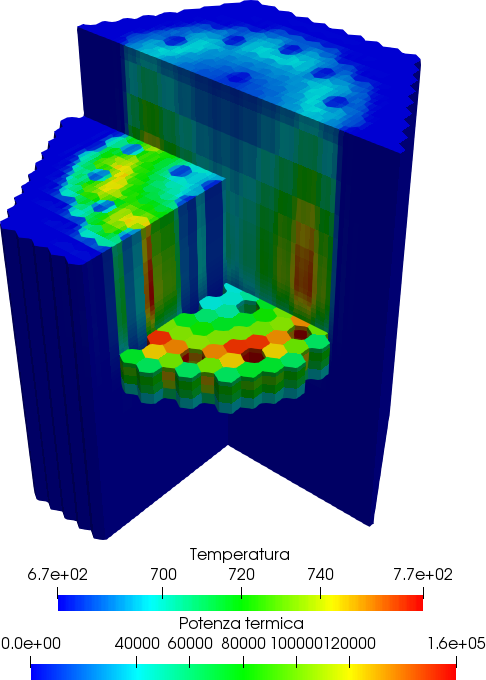
\includegraphics[width=0.32\textwidth]{./figure/result_tred/new/tred2-temp.png}
}
\hspace{1.2cm}
\subfigure[Step temporale 2]
{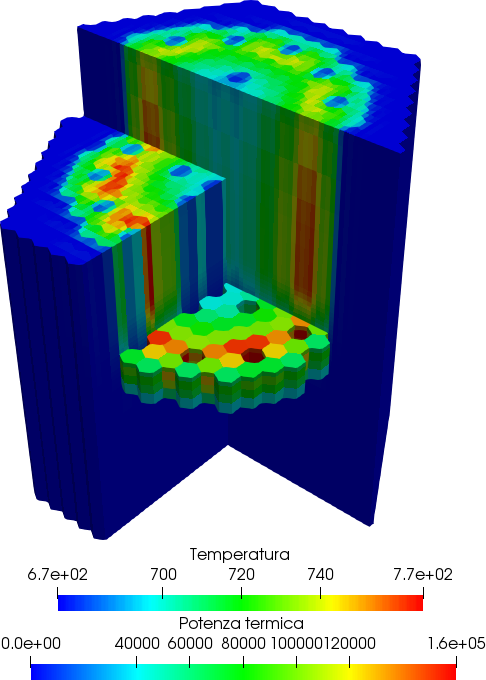
\includegraphics[width=0.32\textwidth]{./figure/result_tred/new/tred3-temp.png}
}\\
\subfigure[Step temporale 3]
{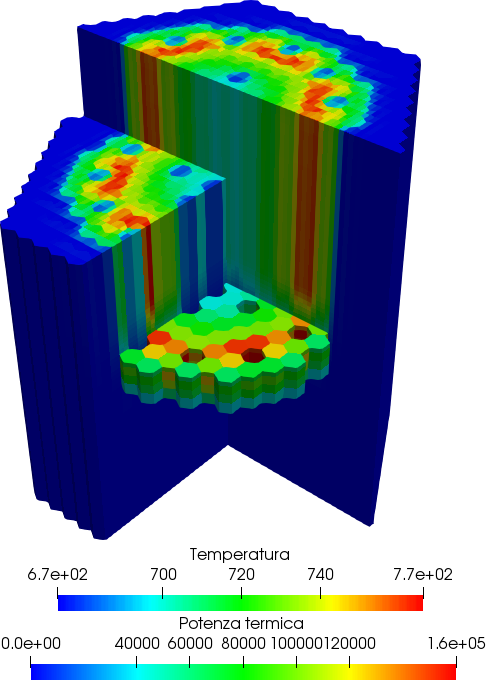
\includegraphics[width=0.32\textwidth]{./figure/result_tred/new/tred1-temp.png}
}
\caption{Distribuzione del campo di temperatura sopra il reattore sezionato con distribuzione di potenza termica su sezione del
nocciolo del reattore. 
\label{temp-tred}}
\end{figure}
%%%%%%%%%%%%%%%%%%%%%%%%%%%%%%%%%%%%%%%
%%%%%%%%%%%%%%%%%%%%%%%%%%%%%%%%%%%%%%%%%%%%%%%%%%%%%%%%
\begin{figure}[!htb]
\centering
\subfigure[$z$=175cm]
{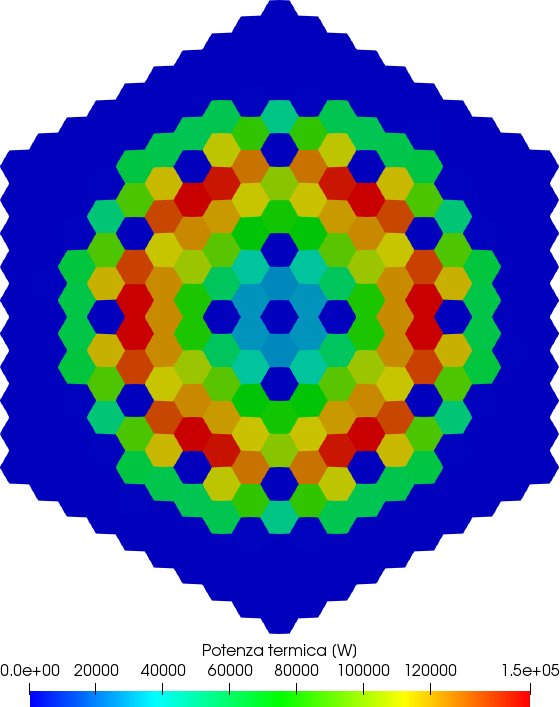
\includegraphics[width=0.28\textwidth]{./figure/result_tred/morenew/slice/pw-175.png}}
\hspace{1.5cm}
\subfigure[$z$=205cm]
{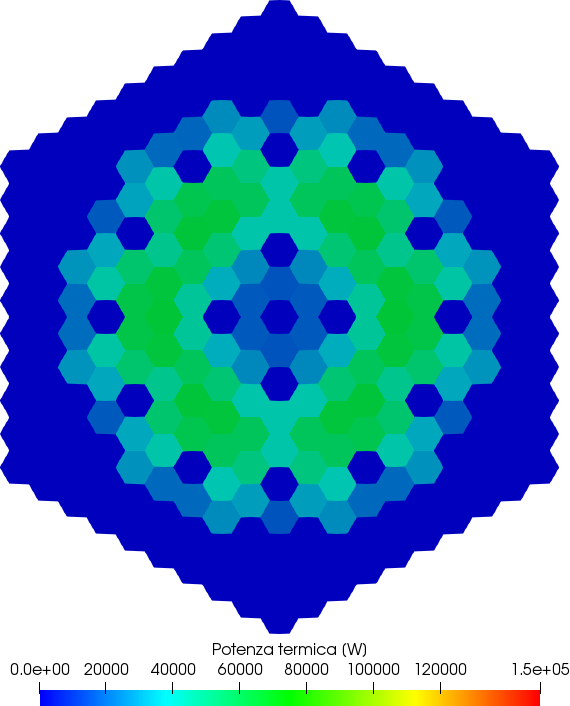
\includegraphics[width=0.28\textwidth]{./figure/result_tred/morenew/slice/pw-205.png}}\\
\subfigure[$z$=175cm]
{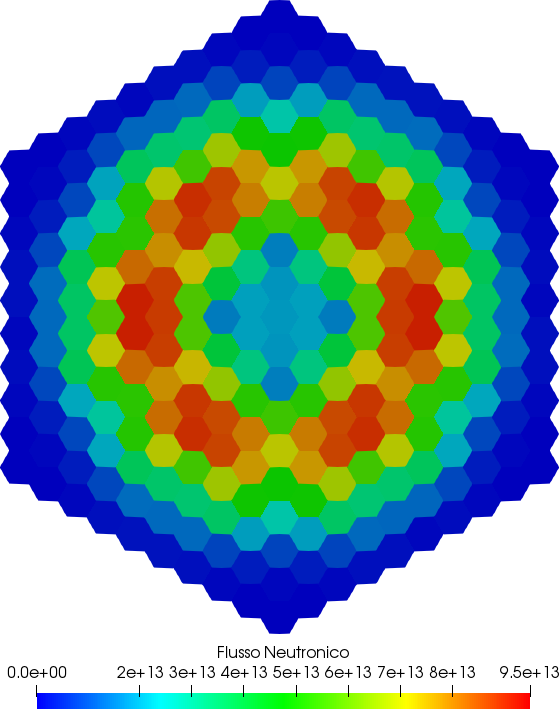
\includegraphics[width=0.28\textwidth]{./figure/result_tred/morenew/slice/flux-175.png}}
\hspace{1.5cm}
\subfigure[$z$=205cm]
{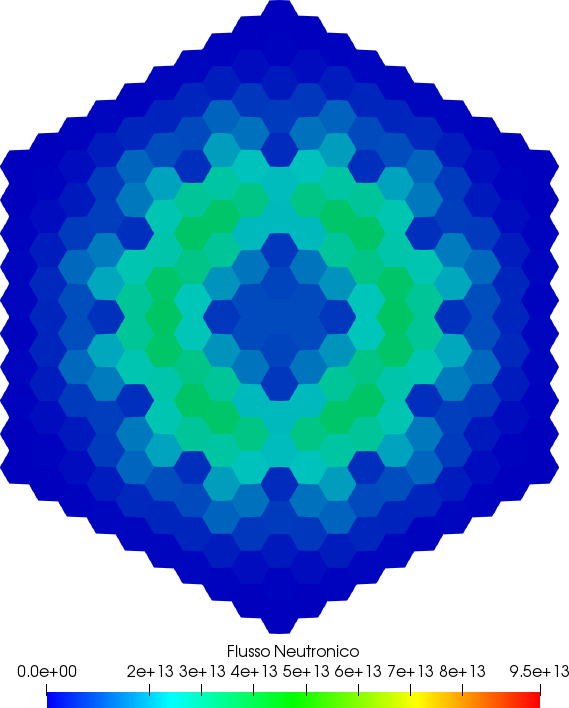
\includegraphics[width=0.28\textwidth]{./figure/result_tred/morenew/slice/flux-205.png}}\\
\subfigure[$z$=175cm]
{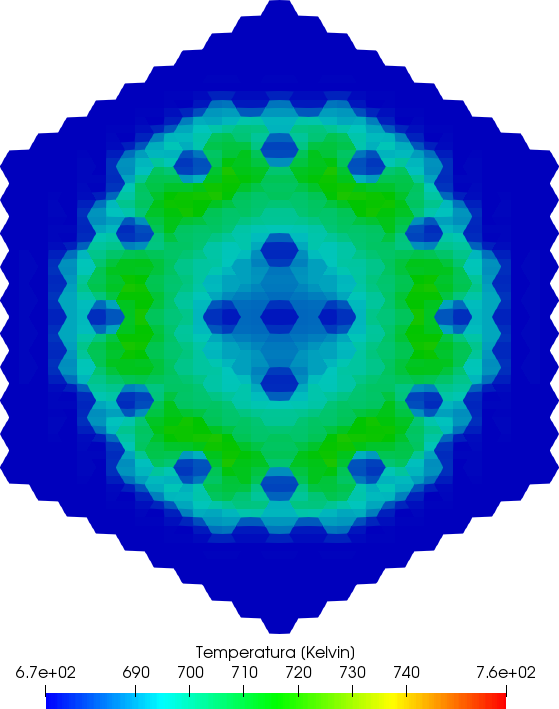
\includegraphics[width=0.28\textwidth]{./figure/result_tred/morenew/slice/temp-175.png}}
\hspace{1.5cm}
\subfigure[$z$=205cm]
{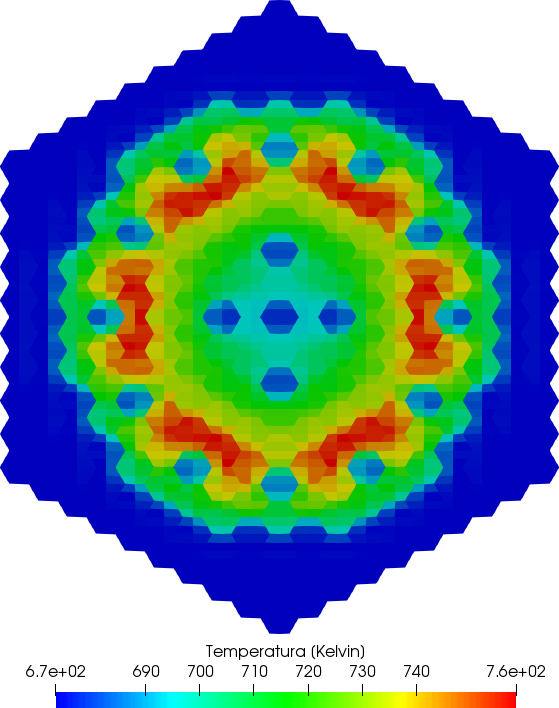
\includegraphics[width=0.3\textwidth]{./figure/result_tred/morenew/slice/temp-205.png}}\\
\caption{Distribuzione radiale di potenza termica (a), (b), di flusso neutronico 
(c), (d), e di temperatura (e), (f) per l'altezza centrale al nocciolo ($z$=175cm) e 
di uscita dal nocciolo ($z$=205cm). \label{slice}}
\end{figure}
%%%%%%%%%%%%%%%%%%%%%%%%%%%%%%%%%%%%%%%%%%%%%%%%%%
\begin{figure}[!htb]
\centering
\subfigure[Sezione cilindrica  \label{sezz}]
{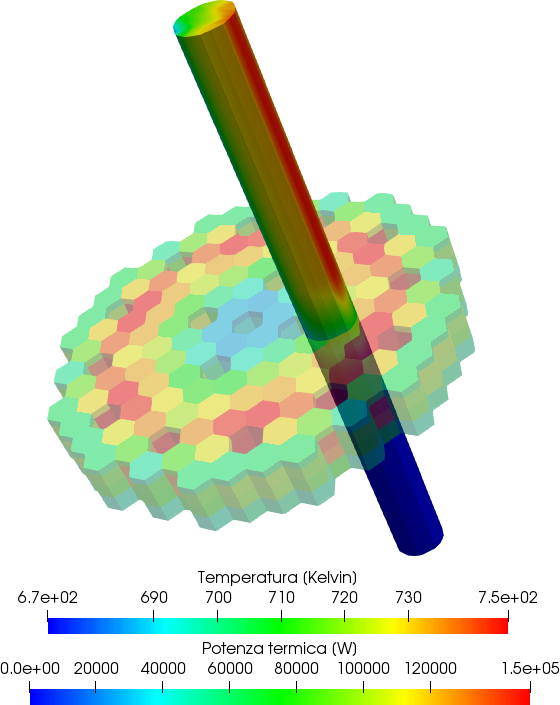
\includegraphics[height=0.3\textheight]{./figure/result_tred/morenew/tempassurda.png}}
\hspace{5mm}
\subfigure[Profilo di temperatura \label{tempz}]
{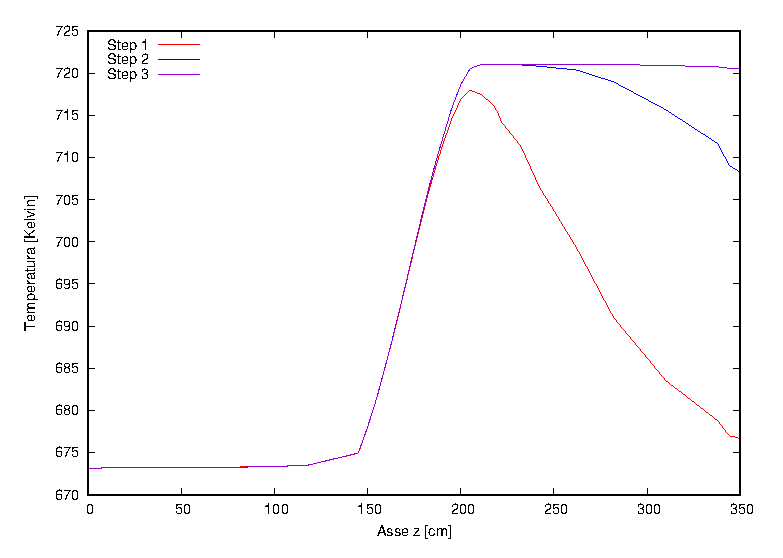
\includegraphics[height=0.25\textheight]{./graph/tempz}}
\caption{Distribuzione di temperatura lungo la coordinata $z$ per una assembly del reattore.}
\end{figure}
%%%%%%%%%%%%%%%%%%%%%%%%%%%%%%%%%%%%%%%%%%%%%%%%%%%%%%%555
Analizzando il caso di fine ciclo considerato come EOC, si confrontano alcuni 
grafici tra il caso in cui le barre di controllo sono inserite e quello in cui 
sono estratte. In Figura \ref{graphfluxy} è rappresentato il grafico della 
distribuzione di flusso neutronico lungo l'asse delle ordinate e all'altezza 
pari a 175cm. La distribuzione del flusso è più intensa nelle regioni dove 
l'arricchimento del combustibile MOX è più alto e l'inserimento delle barre di 
controllo e di sicurezza crea una depressione più marcata al centro del 
nocciolo, per via delle reazioni d'assorbimento da parte del boro contenuto 
nelle barre di sicurezza.

Allo stesso modo, in Figura \ref{graphpowery}, sono rappresentate le 
distribuzioni di potenza termica espressi in Watt lungo l'asse delle ordinate e 
passante per il centro del reattore, in modo da valutare l'effettiva potenza 
termica rilasciata dagli assembly di combustibile all'interno del nocciolo in 
funzione dell'inserimento o meno delle barre di controllo.
Alcuni valori di interesse per la valutazione del reattore nucleare, considerando 
sempre la contrapposizione tra barre inserite e barre estratte, sono tabulate 
in Tabella \ref{paraminseextr}. Si nota che le differenze della potenza per i vari casi.

%%%%%%%%%%%%%%%%%%%%%%%%%%%%%%%%%%%%%%%%%%%%%%%%%%%%%%%%%%%%%%%%%%%%%%%%%%%%%%%5
La suddivisione dei gruppi energetici è stata valutata anche per condensazione a 
5 gruppi di energia. Purtroppo i calcoli di reattori che derivano da questa 
condensazione sono risultati abbastanza approssimativi anche se il tempo 
computazionale risultava drasticamente ridotto.
Tuttavia la suddivisione a 33 gruppi ha permesso la valutazione anche dello 
spettro neutronico in base alle energie.
Ricordando che si considera zona termica le energie comprese tra 
0.001eV - 0.625eV, la zona epitermica tra 0.625eV - 300keV e la zona veloce 
300keV - 10MeV, i 33 gruppi ottenuti appartengono: da 1 a 9 alla zona veloce, da 
10 a 31 alla zona epitermica, e da 32 a 33 alla zona termica.
Più precisamente gli intervalli energetici sono tabulati in Tabella 
\ref{groupenergy}, in cui sono espressi anche il flusso neutronico medio nella 
zona del combustibile per i vari gruppi di energia, considerando le barre 
inserite e il tempo di fine ciclo (EOC).
Inoltre a seguito della Tabella \ref{groupenergy}, in Figura \ref{energyy} sono 
stati graficati la distribuzione del flusso neutronico per alcuni gruppi di 
energia lungo l'asse dell'ordinate. Si nota come lo spettro neutronico sia 
prevalentemente concentrato nella zona veloce e nella zona epitermica più 
energetica.

Attraverso la piattaforma numerica, l'accoppiamento tra la neutronica e la 
termo-idraulica permette la stampa delle distribuzioni di potenza termica, sia 
normalizzata che non, del flusso neutronico, sia medio che a gruppi, e del campo 
di temperatura.
Grazie alle capacità offerte dal software integrato \textit{ParaView}, è possibile 
ottenere la visualizzazione tridimensionale delle grandezze appena citate.
Il campo di temperatura è risolto attraverso lo scambio della sorgente termica 
ottenuta dal codice neutronico dopo aver risolto il calcolo del flusso neutronico.
%%%%%%%%%%%%%%%%%%%%%%%%%%%%%%%%%%%%%%%%%%%%%5
In Figura \ref{nocflux} sono mostrate le stampe del flusso neutronico sulla 
sezione e il nocciolo del reattore in funzione delle barre di controllo. Si nota 
una maggiore uniformità del flusso neutronico quando le barre sono estratte. 
Questo è dovuto in particolare al fatto che le barre di controllo assorbono una 
parte della popolazione neutronica rendendo il flusso più concentrato in certe 
regioni.
%%%%%%%%%%%%%%%%%%%%%%%%%%%%%%%%%%%%%%%%%%%%%%%%%%%%%%%%%%%%%%%%%
Di conseguenza anche la potenza termica segue l'andamento del flusso a seguito 
della presenza delle barre di controllo, in quanto la potenza termica e il 
flusso termico sono strettamente legati.
In particolare la potenza termica è stata ottenuta solo per gli assembly di 
combustibile e sono stampati sulla sezione e sul nocciolo del reattore in 
funzione confrontando il comportamento con le barre inserite ed estratte, come 
mostrato in Figura \ref{nocpw}.

In Figura \ref{temp-tred}, invece è rappresentata la distribuzione del campo di 
temperatura sopra il reattore, dove il nocciolo del reattore è visualizzato al 
fine di esprimere la potenza termica. Si nota come a diversi istanti temporali la 
temperatura aumenta nella direzione assiale, in quanto il modello termoidraulico 
è stato considerato come canali chiusi, in cui scorre il fluido refrigerante.
La temperatura in ingresso è stata impostata a 400$^\circ$C e la temperatura in 
uscita ottenuta è di 520$^\circ$C, che risulta perfettamente in linea con i dati 
progettuali ipotizzati per ALFRED; si deduce che il salto di temperatura massimo tra 
ingresso e uscita è di 120$^\circ$C.
Pertanto questi risultati, seppur preliminari e molto semplificati, 
corrispondono alla temperatura di uscita di progetto ipotizzata per il reattore 
ALFRED.

Nella Figura \ref{slice}, è mostrata una matrice di figure che rappresenta la 
distribuzione di potenza termica, di flusso neutronico e di temperatura 
considerando il caso in cui le barre di controllo e di sicurezza siano inserite 
per due altezze che corrispondono al centro del nocciolo, per $z$=175cm, e 
all'uscita del nocciolo, per $z$=205cm.
La distribuzione di temperatura del refrigerante è molto più alta all'uscita del 
nocciolo in quanto il piombo acquista energia attraverso la potenza termica 
generata dagli assembly di combustibile man mano che esso attraversa il 
nocciolo.
In Figura \ref{sezz} è rappresentata una sezione cilindrica del reattore
lungo la coordinata $z$ su cui è visualizzata la distribuzione di temperatura
e la sezione del nocciolo su cui si intravede la distribuzione di potenza 
termica. \`E  stato considerato l'istante temporale in cui la temperatura raggiunge la stazionarietà.
Per questa sezione sono anche mostrati gli andamenti del profilo di temperatura lungo la coordinata 
assiale $z$ nel grafico di Figura \ref{tempz}, dove sono stati effettuati per tre istanti temporali 
differenti. Si nota che il profilo di temperatura ha un incremento nella zona dove è presente il
combustibile, per via della generazione di potenza termica, e durante l'evoluzione temporale il 
refrigerante asporta calore aumentando la sua temperatura; il salto di temperatura della 
sezione cilindrica considerata è di circa 50$^\circ$C.

Infine bisogna sottolineare come questo modello sia semplificato ed i calcoli
non hanno la pretesa di essere risolutivi per la progettazione del reattore ALFRED
appartenente al progetto LEADER. Tuttavia la piattaforma numerica con l'integrazione del
codice di reattore \textit{Donjon} e del codice termoidraulico \textit{FEMuS}, 
permette un'analisi in ambito nucleare facilmente gestibile, 
come riportato dai risultati appena descritti. Inoltre la visualizzazione grafica dei dati dei 
principali parametri di interesse, quali la distribuzione di potenza termica, di flusso neutronico
e di temperatura, consente un interessante approccio multifisico quantitativo.




